\documentclass[11pt]{article}
\usepackage[a4paper,margin=2.6cm]{geometry}
\usepackage[T1]{fontenc}
\usepackage{lmodern}
\usepackage{microtype}
\usepackage{amsmath,amssymb,amsthm,mathtools}
\usepackage{booktabs,tabularx,multirow}
\usepackage{xcolor}
\usepackage[colorlinks=true,linkcolor=accent,citecolor=accent,urlcolor=accent]{hyperref}
\usepackage{algorithm}
\usepackage{algpseudocode}
\usepackage{pgfplots}
\usepackage{caption}
\usepackage{enumitem}
\pgfplotsset{compat=1.17}
\definecolor{accent}{HTML}{1F5FA8}
\definecolor{muted}{HTML}{6B7280}
\definecolor{warm}{HTML}{C2410C}
\captionsetup{font=small,labelfont=bf}
\setlist{itemsep=2pt,topsep=4pt}

\newtheorem{hypothesis}{Hypothesis}
\theoremstyle{definition}
\newtheorem{definition}{Definition}
\newcommand{\E}{\mathbb{E}}
\newcommand{\Var}{\operatorname{Var}}
\newcommand{\argmax}{\operatorname*{arg\,max}}
\newcommand{\1}{\mathbf{1}}
\newcommand{\cfg}[1]{\texttt{\small #1}}

\title{\textbf{Accrete: Production Creates the Conditions for Culture}\\[4pt]
\large Ecological determination of aggregation, the extent of the market, and\\
payoff-biased learning in a deterministic belief-driven agent society}
\author{Accrete project}
\date{November 2026 \quad\textcolor{muted}{(working paper; results from commit \texttt{research/*})}}

\begin{document}
\maketitle

\begin{abstract}
\noindent
We study the emergence of social and economic structure in \emph{Accrete}, a bit-reproducible agent-based model in which about one hundred founders, and their descendants, act only on what they have perceived and remember. Households, hamlets, trails, barter and prices are never scripted; every rule is one agent's preference, perception or ability. We report four results, each from paired multi-seed experiments with explicit uncertainty.
\textbf{(i)}~A Sobol' global sensitivity analysis shows that spatial aggregation is \emph{ecologically} determined: food regrowth and the land-perception threshold carry total-order indices of $0.75$ and $0.22$ for the Clark--Evans ratio, while the sociability and kin preferences, motives added to produce aggregation, carry $0.02$ and $0.03$.
\textbf{(ii)}~Introducing a durable crafted good (tools) multiplies barter about tenfold, grows the monthly trade network from $33$ to $374$ distinct pairs, and raises household wealth inequality (Gini $0.33\!\to\!0.39$, non-overlapping intervals).
\textbf{(iii)}~A division of labour does \emph{not} emerge, under increasing returns to crafting or under stone scarcity. Scarcity suppresses the tool economy rather than concentrating it, which is consistent with Smith's dictum that the division of labour is limited by the extent of the market, here the rate of co-located encounters.
\textbf{(iv)}~Payoff-biased social learning has no effect on trait geography in the baseline economy, where payoffs depend on location rather than behaviour. Once tools make payoffs trait-sensitive, the \emph{same} learning rule raises spatial autocorrelation of all four personality traits ($\Delta I \in [+0.07, +0.12]$, $n=15$ paired seeds, all surviving Holm correction), without changing population, trade or inequality. In this model production does not merely add wealth: it creates the conditions under which cultural transmission becomes visible.
\end{abstract}

\tableofcontents
\newpage

%=====================================================================
\section{Introduction}

Agent-based models of early settlement have a long history, from Schelling's segregation model~\cite{schelling1971} through Sugarscape~\cite{epstein1996} to empirically calibrated reconstructions such as the Artificial Anasazi~\cite{axtell2002} and the Village Ecodynamics project~\cite{kohler2012}. A recurring difficulty is that the structures of interest (villages, markets, cultural regions) are easy to \emph{build in} and hard to \emph{grow}. When a model contains a rule such as ``form a village when $N$ agents are close'', its villages tell us about the rule, not about villages.

Accrete adopts a strict constructive discipline (Section~\ref{sec:principles}): agents decide only from their own fixed-size memory and local perception, and no rule may read a collective quantity. Within that discipline we ask a single question:

\begin{quote}
\emph{Which features of the environment and of individual motivation are necessary and sufficient for durable social and economic structure to emerge from local, belief-driven decisions?}
\end{quote}

\paragraph{Contributions.}
\begin{enumerate}
\item A fully specified, deterministic, cross-platform bit-identical model with a conservation ledger and a belief/truth separation enforced in code (Sections~\ref{sec:model}--\ref{sec:repro}).
\item An \emph{observatory} of measurement-only statistics (spatial point pattern, spatial autocorrelation of traits, inequality, trade-network topology, specialisation) that agents can never read (Section~\ref{sec:measure}).
\item A statistical protocol for stochastic simulators: paired seeds, $t$-intervals, Saltelli--Jansen Sobol' indices with bootstrap intervals, and a \emph{noise share} that flags indices dominated by seed noise (Section~\ref{sec:stats}).
\item Four substantive results (Section~\ref{sec:results}), two of them initially null and then resolved by a theoretically motivated intervention.
\end{enumerate}

%=====================================================================
\section{Design principles}\label{sec:principles}

\begin{enumerate}[label=\textbf{P\arabic*.}]
\item \textbf{Motives, never outcomes.} Every rule is expressible as one agent's preference, perception or ability using only that agent's knowledge. No rule reads settlements, the road network, population statistics or metrics.
\item \textbf{Belief versus truth.} Decisions read the agent's own tile, the static terrain of tiles it knows, its own household, and memory ``as last seen''. Routes are planned over believed terrain.
\item \textbf{Propose, then resolve.} All agents propose against a read-only world; contested actions are resolved by rules that do not favour low identifiers.
\item \textbf{Conservation.} Every unit of food, wood, stone and tools is accounted for as gathered, regrown, eaten, transferred, spoiled, or consumed in construction.
\item \textbf{Reproducibility.} Results are bit-identical across operating systems, CPU architectures and build profiles.
\item \textbf{Inert extensions.} Every new mechanism ships behind a default-off switch; with the switch off, every pre-existing daily metric is bit-identical to the previous build.
\end{enumerate}

%=====================================================================
\section{The model}\label{sec:model}

We follow the spirit of the ODD protocol~\cite{grimm2020}. Time is discrete: one tick is one hour, and $24$ ticks make a day. Configuration values are per day and are converted to per-tick rates in exactly one place.

\subsection{World}
The world is a $W\times H$ grid of tiles $x$, generated procedurally from the seed (elevation, moisture, rivers and biomes). Each land tile has a static fertility $\phi_x\in[0,1]$, a food capacity $K^F_x$ and a wood capacity $K^W_x$, and stone deposits where a noise field exceeds a threshold $\theta_S$. Standing food regrows logistically toward capacity once per day:
\begin{equation}
F_x \leftarrow \min\!\Big(K^F_x,\; F_x + \rho\,\phi_x\,(K^F_x - F_x)\,D_x(t)\Big),
\label{eq:regrow}
\end{equation}
where $\rho$ is \cfg{resources.food\_regrowth} and $D_x(t)\in[0,1]$ is a drought factor. Wood follows \eqref{eq:regrow} with its own rate and no fertility term. Stone does not regrow.

\subsection{Agents}
Agent $i$ carries:
\begin{itemize}
\item needs: hunger $h_i$, energy $e_i$, health $H_i$;
\item an inventory $\mathbf{x}_i\in\mathbb{R}^4_{\ge0}$ over food, wood, stone and tools, with a weight limit;
\item traits $\boldsymbol{\tau}_i=(\text{curiosity},\text{caution},\text{sociability},\text{diligence})\in[0,1]^4$;
\item one gathering skill per natural resource, plus a crafting skill;
\item a fixed-size memory $\mathcal{M}_i$;
\item an optional home.
\end{itemize}

\paragraph{Needs.} Per tick, hunger rises by $\eta_h = 0.33/24$ (halved for juveniles). Eating one unit of food lowers hunger by $0.165$, up to four units per meal. Energy falls by $0.05$ per active tick and recovers by $0.10$ per resting tick ($0.125$ at home). Health falls by $0.05$ per deprived day and $0.15$ per starving day, and recovers by $0.10$ per day otherwise. Frailty accumulates with deprivation, crowding and old age, and death occurs when health reaches zero.

\paragraph{Skills.} A skill has level $\ell = a + p$, where the aptitude $a\sim U[0.7,1.3]$ is fixed at birth and the practice $p$ rises by $\pi$ per productive tick, up to $p_{\max}$, and decays by $0.001$ per idle day. Aptitudes are drawn from named random streams, except the crafting aptitude, which is a stateless hash of $(\text{seed},i)$ so that enabling tools cannot shift any other draw.

\paragraph{Experienced return.} Each agent tracks its foraging return as an exponential moving average, updated daily when it foraged for at least two ticks:
\begin{equation}
r_i \leftarrow 0.8\,r_i + 0.2\,\frac{\text{food gathered today}}{\text{foraging ticks today}}.
\label{eq:return}
\end{equation}
This is the only payoff signal agents exchange (Section~\ref{sec:culture}).

\subsection{Perception and memory}
An agent sees tiles within a terrain-dependent sight radius, subject to line of sight. Its memory holds 64 resource slots partitioned by type (food 40, wood 16, stone 8), 32 trail and road slots, a disruption pool, known homes, reciprocity scores toward up to 32 partners, and a scalar belief $\hat p_i$ about the price of tools. Partitioning matters: a single shared pool let abundant wood evict every food memory, and agents starved beside food.

\subsection{Decision}
Every tick each agent scores a finite set of candidate options $o$, each a goal and a target such as eat, rest, gather food, explore along a ray, establish a home, deposit, craft or reproduce. The score of an option is a sum of \emph{named} terms, which keeps every decision explainable:
\begin{equation}
U_i(o) \;=\; \sum_{k} u_{k}(o;\,\mathcal{M}_i,\boldsymbol{\tau}_i,\text{needs}_i) \;-\; c\,T_i(o) \;+\; \kappa\,\1[o = o_i^{\text{prev}}] \;+\; \varepsilon(i,t,o),
\label{eq:utility}
\end{equation}
where:
\begin{itemize}
\item $T_i(o)$ is the believed travel and work time in ticks, and $c = 0.02$;
\item $\kappa=0.15$ is a commitment bonus that suppresses dithering;
\item $\varepsilon$ is tie-breaking jitter, a stateless hash of $(i,t,\text{goal},\text{target})$ mapped to $[-0.01, 0.01]$, so that no random numbers are drawn and evaluation order is irrelevant.
\end{itemize}
The agent chooses $o_i^\star = \argmax_o U_i(o)$.

Need-driven terms are gated by thresholds that are affine in traits. For example, the eating threshold is $\theta^{\text{eat}}_i = 0.4 - 0.15\,\text{caution}_i$, and the rest threshold falls with diligence, $\theta^{\text{rest}}_i = 0.3 - 0.15\,\text{diligence}_i + \dots$. The food-reserve target grows with caution, $R_i = (2 + 4\,\text{caution}_i)$ days of consumption, and exploration value scales with curiosity and with \emph{desperation} when no food is remembered.

\paragraph{Homes.} Home-site choice combines remembered food within a radius (``site food per person'', \cfg{homes.site\_food\_per\_person}), proximity to known homes (sociability weight $w_s$), proximity to kin (kin weight $w_k$), and a crowding penalty. A move happens only when the best site beats the current one by a margin. These are the levers whose influence Section~\ref{sec:e1} quantifies.

\subsection{Movement}
Each tick gives $10$ movement points, and entering a tile costs a terrain-dependent number of points, lowered by trails and roads. Routes are planned with A$^\ast$ over the agent's \emph{believed} map, so unknown tiles are impassable for planning. Route disruptions (floods, blockages) raise entry costs. An agent standing in a blocked area may step out of it.

\subsection{Resolution of contested actions}
When several agents request $q_1,\dots,q_m$ units from a tile holding $A$, agent $j$ receives
\begin{equation}
g_j = q_j\cdot\min\!\Big(1,\; \frac{A}{\sum_k q_k}\Big),
\end{equation}
which is independent of processing order. Household actions are settled in a permutation drawn from the \cfg{conflicts} stream, and births in parent-identifier order.

\subsection{Reproduction}
An adult with a home may choose to reproduce when it is off cooldown (30 days), healthy, and food-secure: it must carry at least $10$ food with at least $20$ stored at home, and its experienced return must be at least $0.85$. The option's utility weighs offspring value against the security shortfall, land pressure and return. A chosen attempt succeeds with probability $0.35$ from the \cfg{life} stream. Newborns inherit each parent trait with jitter $\pm0.1$ and inherit part of the parent's memory.

\subsection{Social exchange}
Agents on the same tile meet every six ticks.

\paragraph{Information sharing.} A teller shares $1 + \lfloor 2\cdot\text{sociability}\rfloor$ remembered food locations, unless the teller distrusts the listener (negative reciprocity).

\paragraph{Barter.} Agent $i$ values a bundle $\mathbf{x}$ with a piecewise-linear utility over wants $\omega_{i,r}$, the quantities it needs of good $r$:
\begin{equation}
V_i(\mathbf{x}) = \sum_{r} w_{i,r}\min(x_r,\omega_{i,r}) + s\sum_r (x_r-\omega_{i,r})^+,
\qquad m_{i,r} = \begin{cases} w_{i,r} & x_r<\omega_{i,r}\\ s & \text{otherwise.}\end{cases}
\label{eq:barter}
\end{equation}
For a proposer $p$ giving good $g$ for good $r$ to partner $q$, the exchange ratio is the mean of the two marginal rates of substitution, adjusted by trust $\in[-1,1]$:
\begin{equation}
\pi = \tfrac12\!\left(\frac{m_{p,g}}{m_{p,r}}+\frac{m_{q,g}}{m_{q,r}}\right)\big(1+\tfrac12\,\text{trust}_{q\to p}\big).
\end{equation}
Over a grid of quantities, the trade chosen maximises $\min(\Delta V_p,\Delta V_q)$ (a maximin bargain), subject to both gains exceeding a minimum and to carrying capacity. Each side then updates reciprocity toward the other by its share of the total gain; reciprocity decays at $0.02$ per day.

\subsection{Trails}
Traffic $\tau_x$ decays daily as $\tau_x\leftarrow0.95\,\tau_x$ plus crossings. A tile becomes a trail when $\tau_x\ge20$, and fades after 30 days below threshold. Roads are \emph{built} by agents when the believed time saved for their household exceeds the labour cost.

\subsection{Tools: a production chain with learned prices}\label{sec:tools}
Tools are a durable good that exists only in inventories, chests and piles.
\begin{itemize}
\item \textbf{Use.} A tool in hand multiplies gathering rates by $\beta=1.5$ and wears by $1/48$ per productive tick.
\item \textbf{Craft.} Crafting takes $4$ ticks, consumes $2$ wood and $1$ stone, and yields $b\cdot\ell^{\text{craft}}_i$ tools, capped by carrying room.
\item \textbf{Motive.} An adult crafts if it holds no tool, or if one batch is believed to fetch at least $4$ food: $\hat p_i\, b\,\ell^{\text{craft}}_i \ge 4$.
\item \textbf{Prices.} Each agent learns the price $\hat p_i$ (food per tool) from its own tool-for-food trades and from conversation:
\begin{equation}
\hat p_i \leftarrow \hat p_i + \lambda\,(p^{\text{obs}} - \hat p_i),\qquad
\hat p_i \leftarrow \hat p_i + \gamma\,(\hat p_j - \hat p_i),
\end{equation}
with $\lambda=0.3$, $\gamma=0.2$ and prior $\hat p=3$.
\end{itemize}
No agent observes a market; any common price is emergent.

\subsection{Payoff-biased social learning}\label{sec:culture}
In the meeting where food locations are shared, each agent also mentions its experienced return \eqref{eq:return}. A listener $i$ who hears a higher return from teller $j$ moves every trait toward the teller's:
\begin{gather}
\boldsymbol{\tau}_i \leftarrow \boldsymbol{\tau}_i + k_{ij}\,(\boldsymbol{\tau}_j - \boldsymbol{\tau}_i),\
k_{ij} = \alpha\,\min\!\Big(1,\frac{r_j - r_i}{r_i}\Big)\big(\tfrac12 + \tfrac12\,\text{sociability}_i\big)\,\1[r_j>r_i],
\label{eq:culture}
\end{gather}
with $\alpha = 0.05$. This is the canonical payoff-biased (``copy the successful'') transmission of Boyd and Richerson~\cite{boyd1985}, restricted to face-to-face contact and to a payoff the listener can actually be told. Genetic inheritance is unchanged.

\subsection{The tick pipeline}

\begin{algorithm}[h]
\caption{One tick of \texttt{Simulation::step}}
\begin{algorithmic}[1]
\State \textbf{observe}: update each agent's memory from its field of view
\State \textbf{plan homes}: re-evaluate home sites, staggered across agents
\State \textbf{propose}: score options \eqref{eq:utility} and plan routes against a read-only world
\State \textbf{resolve}: settle contested gathering, household actions and births
\State \textbf{apply}: move, gather, eat, build, craft; record every flow in the ledger
\State \textbf{deaths}: remove the dead and transfer their goods to home or tile
\State \textbf{meetings}: sharing, barter \eqref{eq:barter}, learning \eqref{eq:culture}, among survivors
\State \textbf{newborns} join
\If{last tick of day} regrowth \eqref{eq:regrow}, spoilage, skill decay, returns \eqref{eq:return}, trails, metrics \EndIf
\end{algorithmic}
\end{algorithm}

%=====================================================================
\section{Determinism and reproducibility}\label{sec:repro}

Bit-identical results on x86-64 and AArch64, in debug and release builds, are obtained by construction:
\begin{itemize}
\item \textbf{Arithmetic.} The core uses only IEEE-754 operations that are correctly rounded: $+,-,\times,\div,\sqrt{\cdot}$, comparisons and casts. Transcendentals, fused multiply--add and the platform hasher are banned by lint, and floats are summed in fixed order and sorted with a total order.
\item \textbf{Randomness.} All randomness comes from named ChaCha streams with fixed identifiers (world, weather, life, conflicts, design, \dots). New per-agent quantities are stateless hashes, so adding a mechanism cannot shift existing draws.
\item \textbf{State hash.} Every state-bearing field is fed into a stable hash, floats by their bit patterns. Golden hashes of the world and of the state at ticks $0$, $100$ and $1000$ are checked in continuous integration on both platforms.
\item \textbf{Manifests.} Every run writes a manifest (config, start, final hash, git commit, lockfile hash), and \texttt{accrete reproduce} re-runs it and checks the final hash.
\item \textbf{Ledger.} For each good, stock at time $t$ equals stock at time $0$, plus gathered and regrown, minus eaten, spoiled and consumed, with transfers netting to zero. A checked mode verifies this every tick.
\end{itemize}
Principle P6 is verified empirically. With tools disabled, all 87 prior daily metric columns are identical to the pre-tools build over 120 days, and with culture disabled, all 94 columns are identical to the tools build.

%=====================================================================
\section{Measurement}\label{sec:measure}

All statistics below are computed by measurement-only code that agents never read (principle P1).

\begin{definition}[Clark--Evans ratio]
For $n$ occupied homes on land area $A$, with $d_i$ the distance from home $i$ to its nearest neighbour,
\[R = \frac{\bar d}{\tfrac12\sqrt{A/n}}.\]
$R<1$ indicates clustering, $R\approx1$ complete spatial randomness and $R>1$ dispersion~\cite{clark1954}.
\end{definition}

\begin{definition}[Spatial autocorrelation of a trait]
For adults $i$ with trait values $y_i$, deviations $z_i=y_i-\bar y$ and weights $w_{ij} = (1+d_{ij})^{-1}\1[d_{ij}\le 8]$ (for $i\ne j$), with $W=\sum_{ij}w_{ij}$, Moran's~$I$~\cite{moran1950} is
\[I = \frac{n}{W}\,\frac{\sum_{i\neq j} w_{ij}\,z_iz_j}{\sum_i z_i^2}.\]
Positive $I$ means neighbours resemble each other. Because traits are inherited and children settle near parents, kinship alone produces $I>0$, and every culture effect is measured as a paired difference against this kinship baseline.
\end{definition}

\begin{definition}[Inequality]
Household wealth $v_h$ is the sum of stored and carried goods of residents, valued in food units. The Gini coefficient of $v_1\le\dots\le v_n$ is
\[G = \frac{\sum_{k}(2k-n-1)\,v_k}{n\sum_k v_k}.\]
\end{definition}

\begin{definition}[Specialisation]
Let $\mathbf{p}_i\in\mathbb{R}^4$ be adult $i$'s practice vector over food, wood, stone and crafting, and $\bar{\mathbf{p}}$ the population mean. Then
\[\Sigma = 1 - \frac1n\sum_i \cos(\mathbf{p}_i,\bar{\mathbf{p}}).\]
$\Sigma=0$ means everyone does the same mix of work, and $\Sigma\to1$ means orthogonal occupations.
\end{definition}

\paragraph{Trade network.} Over a rolling 30-day window of executed barters, we measure the number of distinct trading pairs, mean degree, the degree Gini, the cross-household share and the repeat share.

\paragraph{Settlements.} Homes are single-linkage clustered at radius 3. A cluster becomes a \emph{hamlet} when it has at least 5 homes and 15 residents and persists for 60 days.

%=====================================================================
\section{Statistical protocol}\label{sec:stats}

\paragraph{Paired designs.} An intervention and its control share the seed, and therefore the world, the founders and the weather. For an outcome $Y$ and seeds $s=1,\dots,n$ we report the mean paired difference $\bar\Delta$ with the interval $\bar\Delta \pm t_{0.975,n-1}\,\hat\sigma_\Delta/\sqrt n$, together with the sign count. When several traits are tested as one family, we apply Holm's step-down correction.

\paragraph{Global sensitivity.} For $k$ parameters scaled to $[0,1]^k$, two $N\times k$ matrices $A,B$ are taken from a Joe--Kuo Sobol' sequence~\cite{joe2008}. $A_B^{(i)}$ is $A$ with column $i$ taken from $B$. With $f$ the seed-averaged outcome and $V=\Var[f]$ over all evaluations, we use the Saltelli~\cite{saltelli2010} first-order estimator and the Jansen~\cite{jansen1999} total-order estimator:
\begin{align}
S_i &= \frac{1}{V}\cdot\frac1N\sum_{j=1}^N f(B)_j\big(f(A_B^{(i)})_j - f(A)_j\big),\\
S_{T,i} &= \frac{1}{V}\cdot\frac1{2N}\sum_{j=1}^N \big(f(A)_j - f(A_B^{(i)})_j\big)^2.
\end{align}
The design has $N(k+2)$ points. Intervals come from a 95\,\% percentile bootstrap over the $N$ rows (1{,}000 resamples, deterministic stream). The implementation recovers the analytic indices of the Sobol' $g$-function to within $0.03$ at $N=4096$.

\paragraph{Noise share.} A stochastic simulator adds seed noise to $f$. We report
\[\nu = \frac{\E_{\text{points}}\big[\widehat\Var(\bar Y_{\text{seeds}})\big]}{V},\]
the share of output variance attributable to seed noise in the seed mean. Indices for outcomes with large $\nu$ are not interpreted.

%=====================================================================
\section{Results}\label{sec:results}

Unless stated, runs last 300 days from 100 founders on independently generated worlds, with random droughts enabled.

\subsection{E1: aggregation is ecologically determined}\label{sec:e1}

\begin{table}[h]
\centering\small
\caption{Total-order Sobol' indices $S_T$ (95\,\% bootstrap CI) for $k=6$ parameters, $N=32$, 2 seeds, 200 days, 512 runs. Columns: food regrowth $\rho\in[0.04,0.2]$; site food per person $\in[3,8]$; reproduction chance $\in[0.15,0.5]$; sociability weight $w_s\in[0,0.8]$; kin weight $w_k\in[0,0.6]$; household concern $\in[0,1]$.}
\label{tab:sobol}
\begin{tabular}{lccccccc}
\toprule
Outcome & $\rho$ & site food & repr. & $w_s$ & $w_k$ & household & $\nu$\\
\midrule
Population & \textbf{0.64} {\scriptsize[.41,.98]} & 0.23 {\scriptsize[.15,.39]} & 0.07 & 0.00 & 0.01 & 0.00 & 0.02\\
Clark--Evans $R$ & \textbf{0.75} {\scriptsize[.47,1.13]} & 0.22 {\scriptsize[.13,.36]} & 0.02 & 0.02 {\scriptsize[.01,.03]} & 0.03 {\scriptsize[.01,.06]} & 0.01 & 0.08\\
Hamlets & 0.51 {\scriptsize[.19,1.6]} & 0.50 {\scriptsize[.21,1.2]} & 0.25 & 0.09 & 0.04 & 0.04 & 0.11\\
Wealth Gini & \textbf{0.73} & -- & -- & -- & -- & -- & --\\
\bottomrule
\end{tabular}
\end{table}

Table~\ref{tab:sobol} shows that the motives designed to produce aggregation (sociability and kin) explain at most about $5\,\%$ of the variance in clustering, even across their whole plausible range. Food productivity and the land-perception threshold explain almost all of it. For hamlets, $S_T \gg S_1$ for both ecological parameters ($0.51$ vs.\ $0.18$ for $\rho$), so hamlet formation is an \emph{interaction}: it needs surplus \emph{and} permissive land perception together, consistent with a threshold phenomenon. At $N=32$ the first-order indices are poorly determined; only total indices are interpreted.

\subsection{E2: a production chain creates exchange and inequality}

\begin{table}[h]
\centering\small
\caption{Tools $\times$ trade $\times$ food regrowth, 5 seeds, 300 days. Mean and 95\,\% CI.}
\label{tab:tools}
\begin{tabular}{cccrrcc}
\toprule
Tools & Trade & $\rho$ & Trades / run & Pairs / 30 d & $\Sigma$ & Gini\\
\midrule
off & on & 0.15 & 431 {\scriptsize[319, 543]} & 33 & 0.0008 & 0.33 {\scriptsize[.31,.35]}\\
on & on & 0.15 & \textbf{4{,}281} {\scriptsize[3160, 5410]} & \textbf{374} & 0.029 & \textbf{0.39} {\scriptsize[.37,.41]}\\
on & off & 0.15 & 0 & 0 & 0.029 & 0.37 {\scriptsize[.33,.40]}\\
off & on & 0.06 & 79 {\scriptsize[52, 107]} & 4 & 0.0002 & 0.31\\
on & on & 0.06 & \textbf{779} {\scriptsize[602, 956]} & \textbf{40} & 0.025 & 0.32\\
\bottomrule
\end{tabular}
\end{table}

Tools raise barter about tenfold at both food levels and grow the network more than tenfold (Table~\ref{tab:tools}). Without a good that is valued differently by different agents, \eqref{eq:barter} has few gains to exploit; with tools, it has many. Inequality rises with tools, and partly even without trade, because tool holders gather $1.5\times$ faster and convert that advantage into stores. Price beliefs settle into a dispersed but correlated distribution (coefficient of variation $\approx0.36$): neither a single market price nor independent guesses.

\subsection{E2b: no division of labour, because the market is too small}

\begin{table}[h]
\centering\small
\caption{Tools on, trade on, $\rho=0.15$. Stone threshold $\theta_S$ (higher means scarcer, more localised stone) $\times$ practice cap $p_{\max}$ (higher means stronger increasing returns to crafting). 5 seeds.}
\label{tab:spec}
\begin{tabular}{ccccccc}
\toprule
$\theta_S$ & $p_{\max}$ & $\Sigma$ & Crafter share & Tool holders & Trades / run & Gini\\
\midrule
0.60 & 0.3 & 0.029 {\scriptsize[.024,.033]} & 0.27\,\% & 46\,\% & 4{,}281 & 0.39\\
0.60 & 1.0 & 0.016 {\scriptsize[.013,.019]} & 0.68\,\% & 48\,\% & 4{,}991 & 0.41\\
0.75 & 0.3 & 0.021 & 0.25\,\% & 30\,\% & 3{,}130 & 0.36\\
0.75 & 1.0 & 0.012 & 0.61\,\% & 32\,\% & 3{,}790 & 0.37\\
0.85 & 0.3 & 0.006 {\scriptsize[.002,.010]} & 0.05\,\% & 9\,\% & 2{,}400 & 0.32\\
0.85 & 1.0 & 0.004 & 0.41\,\% & 11\,\% & 2{,}780 & 0.34\\
\bottomrule
\end{tabular}
\end{table}

We predicted that either intervention would produce specialists. Neither did (Table~\ref{tab:spec}):
\begin{itemize}
\item Increasing returns raise the crafter share about $2.5\times$, but it stays below $1\,\%$ of adults, and overall specialisation \emph{falls}, because the few long-practised crafters pull the mean vector toward crafting.
\item Scarce stone does not create stone or tool specialists. It shrinks the whole tool economy: tool holders fall from $46\,\%$ to $9\,\%$, and trade and inequality fall with them.
\end{itemize}
The binding constraint is not the production technology but \emph{finding a counterparty}. Barter happens only between co-located agents, every six ticks, and agents keep no memory of who sells what. In Smith's terms~\cite{smith1776}, the division of labour is limited by the extent of the market, and here the market extends exactly as far as an agent's daily encounters. This makes a sharp, testable prediction: a perceptual or mnemonic channel for ``who has what'' (memory of past trading partners and their goods, or a meeting place that agents learn to visit) should produce specialisation where technology alone did not.

\subsection{E5: production creates the conditions for culture}

\begin{hypothesis}[H5]
Payoff-biased learning \eqref{eq:culture} produces cultural regions: spatial autocorrelation of traits above the kinship baseline.
\end{hypothesis}

\begin{table}[h]
\centering\small
\caption{Paired effect of culture on Moran's $I$ of each trait (culture minus control, same seed), with and without tools. 95\,\% $t$-interval, sign count, and Holm-adjusted significance over the four traits.}
\label{tab:culture}
\begin{tabular}{lcccc}
\toprule
& \multicolumn{2}{c}{Tools off ($n=5$)} & \multicolumn{2}{c}{Tools on ($n=15$)}\\
\cmidrule(lr){2-3}\cmidrule(lr){4-5}
Trait & $\Delta I$ & up & $\Delta I$ & up\ \ ($p$)\\
\midrule
Caution & $+0.002$ {\scriptsize[$-.14$, $+.15$]} & 3/5 & $\mathbf{+0.122}$ {\scriptsize[$+.053$, $+.190$]} & 13/15\ \ (0.002)\\
Curiosity & $+0.030$ {\scriptsize[$-.05$, $+.12$]} & 3/5 & $\mathbf{+0.092}$ {\scriptsize[$+.032$, $+.151$]} & 13/15\ \ (0.005)\\
Sociability & $-0.024$ {\scriptsize[$-.13$, $+.08$]} & 2/5 & $\mathbf{+0.113}$ {\scriptsize[$+.059$, $+.166$]} & 13/15\ \ (0.0005)\\
Diligence & $+0.099$ {\scriptsize[$-.16$, $+.36$]} & 3/5 & $\mathbf{+0.074}$ {\scriptsize[$+.013$, $+.136$]} & 12/15\ \ (0.022)\\
\midrule
Population & $-13$ {\scriptsize[$-42$, $+16$]} & & $-4$ {\scriptsize[$-35$, $+28$]} & \\
Wealth Gini & $-0.014$ & & $+0.006$ {\scriptsize[$-.010$, $+.021$]} & \\
Clark--Evans $R$ & $+0.014$ & & $+0.005$ {\scriptsize[$-.029$, $+.040$]} & \\
\bottomrule
\end{tabular}
\end{table}

\begin{figure}[h]
\centering
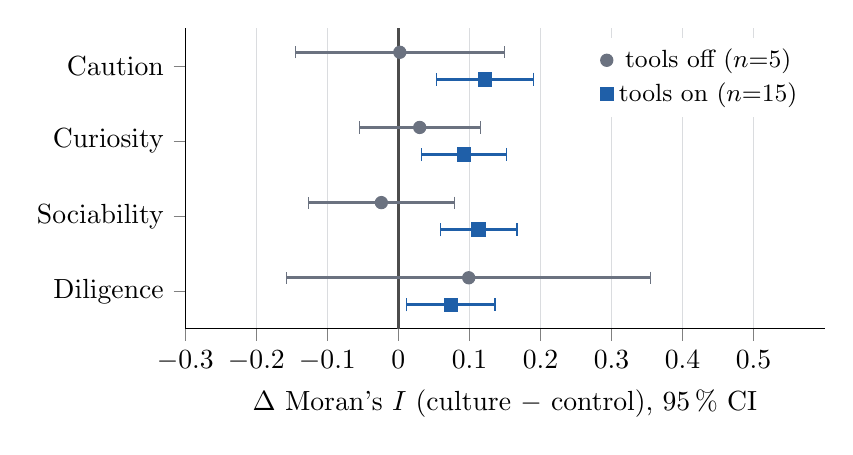
\begin{tikzpicture}
\begin{axis}[
  width=0.8\linewidth, height=5.4cm, y dir=reverse,
  xmin=-0.3, xmax=0.6, ymin=0.5, ymax=4.5,
  ytick={1,2,3,4}, yticklabels={Caution,Curiosity,Sociability,Diligence},
  xtick={-0.3,-0.2,-0.1,0,0.1,0.2,0.3,0.4,0.5},
  xticklabel style={/pgf/number format/fixed,/pgf/number format/precision=1},
  xlabel={$\Delta$ Moran's $I$ (culture $-$ control), 95\,\% CI},
  legend style={at={(0.98,0.97)},anchor=north east,font=\small,draw=none,fill=white},
  axis lines*=left, xmajorgrids, grid style={muted!25}, tick align=outside,
]
\draw[black!70,thick] (axis cs:0,0.5) -- (axis cs:0,4.5);
\addplot+[only marks, mark=*, mark size=2.2pt, color=muted, mark options={fill=muted},
  error bars/.cd, x dir=both, x explicit, error bar style={line width=1pt}]
  coordinates {(0.002,0.82) +- (0.147,0) (0.030,1.82) +- (0.085,0) (-0.024,2.82) +- (0.103,0) (0.099,3.82) +- (0.256,0)};
\addplot+[only marks, mark=square*, mark size=2.4pt, color=accent, mark options={fill=accent},
  error bars/.cd, x dir=both, x explicit, error bar style={line width=1.2pt}]
  coordinates {(0.122,1.18) +- (0.068,0) (0.092,2.18) +- (0.060,0) (0.113,3.18) +- (0.054,0) (0.074,4.18) +- (0.062,0)};
\legend{tools off ($n{=}5$), tools on ($n{=}15$)}
\end{axis}
\end{tikzpicture}
\caption{The same learning rule is inert in a foraging economy and creates trait geography in a production economy.}
\label{fig:culture}
\end{figure}

In the baseline foraging economy, H5 fails despite a large learning dose ($\approx27{,}000$ copying events per run, $0.27$ per person-day): every interval spans zero. The explanation is visible in E1: an agent's return \eqref{eq:return} is governed by where it lives (land quality and local competition), not by its traits, so copying the successful copies \emph{luck}, and the transmitted variants are nearly selectively neutral. Payoff-biased transmission builds adaptive culture only when payoffs covary with the transmitted behaviour~\cite{boyd1985,henrich2004}.

Tools make payoffs trait-sensitive. Diligence and caution shape how agents accumulate the wood and stone a tool requires, and a tool multiplies foraging return by $1.5$. Under tools, the identical rule raises spatial autocorrelation of all four traits (Table~\ref{tab:culture}, Figure~\ref{fig:culture}). All four effects survive Holm correction at $\alpha=0.05$, and 12--13 of 15 seeds move in the predicted direction. Population, inequality, trade volume and clustering are unchanged, so culture reorganises \emph{who lives near whom} without altering the economy's size or distribution.

An exploratory increase in hamlets under culture without tools ($+0.8$, 5 seeds) did not replicate under tools ($-0.7$ {\scriptsize[$-1.7$, $+0.2$]}, 15 seeds) and is not claimed.

%=====================================================================
\section{Discussion}

\paragraph{A layered causal picture.} The results compose into a hierarchy:
\begin{enumerate}
\item \textbf{Ecology} sets how many people there are and how they cluster (E1).
\item \textbf{Production technology} sets whether exchange has gains, and therefore the density of the social network and the level of inequality (E2).
\item The \textbf{extent of encounters} bounds the division of labour (E2b).
\item \textbf{Culture} becomes visible only once production makes behaviour matter to payoff (E5).
\end{enumerate}
Social preferences sit at the bottom of the variance budget throughout. This ordering echoes materialist accounts in archaeology and cultural ecology, but here it is derived, not assumed: none of these dependencies is written into any rule.

\paragraph{Why the nulls matter.} Two hypotheses (H2 specialisation, H5 culture) failed in their first form, and in both cases the failure pointed to a precise missing condition. The second form of H5 then succeeded. A model that cannot fail cannot teach, and principle P1 (motives, never outcomes) is what makes these failures informative.

\paragraph{Limitations.}
\begin{itemize}
\item The pilot Sobol' study uses $N=32$ and 2 seeds; first-order indices are not resolved, and the noise share is high for foraging radius and Moran's $I$.
\item Population is about $500$, so ``hamlets'' are tens of people, and claims about towns or states are out of scope.
\item Parameters are plausible but not calibrated against an archaeological record.
\item The mechanism proposed for E5 (trait-sensitive payoffs) is consistent with the data but not isolated. A direct test would log the regression slope of $r_i$ on $\boldsymbol\tau_i$ with and without tools.
\end{itemize}

\paragraph{Next experiments.}
\begin{enumerate}
\item \textbf{Market extent:} give agents memory of past partners' surplus goods, and test whether $\Sigma$ rises (the Smithian prediction).
\item \textbf{Payoff--trait slope:} measure $\partial r/\partial\boldsymbol\tau$ directly and show that the culture effect scales with it.
\item \textbf{A full Sobol' study} at $N\ge128$ with 5 seeds, adding the tools and culture parameters.
\item \textbf{A phase diagram} of hamlet formation over $(\rho, \text{site food})$, to locate the threshold implied by $S_T\gg S_1$.
\end{enumerate}

%=====================================================================
\section{Reproducing the results}

\begin{small}
\begin{verbatim}
accrete sweep --sobol 32 --param resources.food_regrowth=0.04..0.2 \
   --param decision.social_weight=0..0.8 --param decision.kin_weight=0..0.6 \
   --param homes.site_food_per_person=3..8 \
   --param infrastructure.household_weight=0..1 \
   --param life.reproduce_chance=0.15..0.5 --seed 1-2 --days 200      # E1
accrete sweep --param tools.enabled=false,true \
   --param social.trade_enabled=false,true \
   --param resources.food_regrowth=0.06,0.15 --seed 1-5 --days 300    # E2
accrete sweep --set tools.enabled=true \
   --param resources.stone_threshold=0.6,0.75,0.85 \
   --param skills.practice_max=0.3,1.0 --seed 1-5 --days 300          # E2b
accrete sweep --set tools.enabled=true --param culture.enabled=false,true \
   --seed 1-15 --days 300                                             # E5
\end{verbatim}
\end{small}
Every run writes a manifest, and \texttt{accrete reproduce <manifest>} verifies its final state hash.

%=====================================================================
\begin{thebibliography}{99}\small
\bibitem{axtell2002} R.~L.~Axtell, J.~M.~Epstein, J.~S.~Dean, et al. Population growth and collapse in a multiagent model of the Kayenta Anasazi in Long House Valley. \emph{PNAS} 99(suppl.~3):7275--7279, 2002.
\bibitem{boyd1985} R.~Boyd and P.~J.~Richerson. \emph{Culture and the Evolutionary Process}. University of Chicago Press, 1985.
\bibitem{clark1954} P.~J.~Clark and F.~C.~Evans. Distance to nearest neighbor as a measure of spatial relationships in populations. \emph{Ecology} 35(4):445--453, 1954.
\bibitem{epstein1996} J.~M.~Epstein and R.~Axtell. \emph{Growing Artificial Societies: Social Science from the Bottom Up}. MIT Press, 1996.
\bibitem{grimm2020} V.~Grimm, S.~F.~Railsback, C.~E.~Vincenot, et al. The ODD protocol for describing agent-based and other simulation models: a second update. \emph{JASSS} 23(2):7, 2020.
\bibitem{henrich2004} J.~Henrich. Demography and cultural evolution. \emph{American Antiquity} 69(2):197--214, 2004.
\bibitem{jansen1999} M.~J.~W.~Jansen. Analysis of variance designs for model output. \emph{Computer Physics Communications} 117:35--43, 1999.
\bibitem{joe2008} S.~Joe and F.~Y.~Kuo. Constructing Sobol' sequences with better two-dimensional projections. \emph{SIAM J.\ Sci.\ Comput.} 30(5):2635--2654, 2008.
\bibitem{kohler2012} T.~A.~Kohler and M.~D.~Varien (eds.). \emph{Emergence and Collapse of Early Villages}. University of California Press, 2012.
\bibitem{moran1950} P.~A.~P.~Moran. Notes on continuous stochastic phenomena. \emph{Biometrika} 37:17--23, 1950.
\bibitem{saltelli2010} A.~Saltelli, P.~Annoni, I.~Azzini, et al. Variance based sensitivity analysis of model output: design and estimator for the total sensitivity index. \emph{Computer Physics Communications} 181:259--270, 2010.
\bibitem{schelling1971} T.~C.~Schelling. Dynamic models of segregation. \emph{J.\ Math.\ Sociology} 1:143--186, 1971.
\bibitem{smith1776} A.~Smith. \emph{An Inquiry into the Nature and Causes of the Wealth of Nations}, Book I, Ch.~3. 1776.
\end{thebibliography}

\end{document}
